\documentclass{article}


% if you need to pass options to natbib, use, e.g.:
%     \PassOptionsToPackage{numbers, compress}{natbib}
% before loading neurips_2024


% ready for submission
% \usepackage{neurips_2024}


% to compile a preprint version, e.g., for submission to arXiv, add add the
% [preprint] option:
%     \usepackage[preprint]{neurips_2024}


% to compile a camera-ready version, add the [final] option, e.g.:
\usepackage[final]{neurips_2024}


% to avoid loading the natbib package, add option nonatbib:
%    \usepackage[nonatbib]{neurips_2024}


\usepackage[utf8]{inputenc} % allow utf-8 input
\usepackage[T1]{fontenc}    % use 8-bit T1 fonts
\usepackage{hyperref}       % hyperlinks
\usepackage{url}            % simple URL typesetting
\usepackage{booktabs}       % professional-quality tables
\usepackage{amsfonts}       % blackboard math symbols
\usepackage{nicefrac}       % compact symbols for 1/2, etc.
\usepackage{microtype}      % microtypography
\usepackage{xcolor}         % colors

\usepackage{bm}
\usepackage{tabularx}
\usepackage{multirow}
\usepackage{xspace}
\usepackage{graphicx}
\usepackage{amsmath}

\newcommand{\sfc}[1]{\textcolor{blue}{#1}}

\newcommand{\subf}[2]{%
  {\footnotesize\begin{tabular}[t]{@{}c@{}}
  #1\\#2
  \end{tabular}}%
}

\newcommand{\ours}{$\texttt{DiffER}$\xspace}


\title{{\ours}: Categorical Diffusion Models for Chemical Retrosynthesis}


% The \author macro works with any number of authors. There are two commands
% used to separate the names and addresses of multiple authors: \And and \AND.
%
% Using \And between authors leaves it to LaTeX to determine where to break the
% lines. Using \AND forces a line break at that point. So, if LaTeX puts 3 of 4
% authors names on the first line, and the last on the second line, try using
% \AND instead of \And before the third author name.


\author{%
  Sean F.~Current \\
  Department of Computer Science \\
  The Ohio Statue University \\
  Columbus, OH 43202 \\
  \texttt{current.33@osu.edu} \\
  \And
  Ziqi Chen \\
  Department of Computer Science \\
  The Ohio Statue University \\
  Columbus, OH 43202 \\
  \texttt{chen.8484@osu.edu} \\
  \And
  Daniel Adu-Ampratwum \\
  College of Pharmacy \\
  The Ohio Statue University \\
  Columbus, OH 43202 \\
  \texttt{adu-ampratwum.1@osu.edu} \\
  \And
  Xia Ning \\
  Department of Computer Science \\
  Department of Biomedical Informatics \\
  The Ohio Statue University \\
  Columbus, OH 43202 \\
  \texttt{ning.104@osu.edu} \\
  \And
  Srinivasan Parthasarathy \\
  Department of Computer Science \\
  The Ohio Statue University \\
  Columbus, OH 43202 \\
  \texttt{srini@cse.ohio-state.edu} \\
 }


\begin{document}


\maketitle


\begin{abstract}
  Methods for automatic chemical retrosynthesis have found recent success through the application of models traditionally built for natural language processing, primarily through transformer neural networks. These models have demonstrated significant ability to translate between the SMILES encodings of chemical products and reactants, but are constrained as a result of their autoregressive nature. We propose \ours, an alternative template-free method for retrosynthesis prediction in the form of categorical diffusion, which allows the entire output SMILES sequence to be predicted in unison. We construct an ensemble of diffusion models which achieves state of the art performance for top-1 accuracy and competitive performance for top-3 and top-5 accuracy. We prove that \ours is a strong baseline for a new class of template-free model and is capable of learning a variety of synthetic techniques used in laboratory settings.
\end{abstract}


\section{Introduction}
\label{sec:intro}

Retrosynthesis prediction is a vital step in organic synthesis tasks, particularly those posed for drug discovery or drug engineering. In forward synthesis prediction, the products of a chemical reaction are predicted from known reactants; retrosynthesis prediction reverses this process, instead predicting possible reactants that would produce a target product. Repeated application of retrosynthesis prediction can help chemists construct synthetic pathways for drug targets \cite{segler2017neural, segler2018planning, shen2021automation}, promoting the discovery and advancement of new pharmaceuticals. While numerous types of models for computer-aided retrosynthesis have been proposed, many modern approaches utilize data-driven machine learning to find suitable models for retrosynthesis prediction.

Recent advances in machine learning models for chemical retrosynthesis have taken advantage of transformer architectures originally crafted for natural language tasks. Instead of operating on natural language, these models are set to operate on SMILES \cite{weininger1988smiles} encodings of chemical products and reactants, effectively translating between two molecular sets \cite{liu2017retrosynthetic}. Indeed, recent work has done precisely this, going as far as using neural machine translation models originally built for language tasks for retrosynthesis prediction \citep{zhong2022root, irwin2022chemformer}. While these models exhibit remarkable performance compared to other baseline methods for retrosynthesis, they impose autoregressive constraints during training and prediction, enforcing sequential decoding of the SMILES string. A more detailed overview of current work in single-step retrosynthesis we compare our work to is provided in Appendix \ref{sec:A1}.

In this work, we offer \ours, an alternative to sequential decoding of SMILES strings in the prediction process by utilizing categorical diffusion models rather than autoregressive models. This exchange allows \ours to decode the entire SMILES string in unison, rather than in an autoregresssive manner. We hypothesize that by allowing the model to predict the entire SMILES string in unison, it may better learn structural relationships within the molecule. Additionally, diffusion models have experienced a recent surge of success for many generation tasks across domains. By employing categorical diffusion for the chemical retrosynthesis task, we provide a strong and competitive baseline for a new class of model. An outline of our approach is display in Figure \ref{fig:schema}, while a more detailed overview is available in Section \ref{sec:methods}. \ours achieves state-of-the-art top-1 accuracy against a variety of baseline models and competitive performance for top-3, top-5, and top-10 accuracy.

\begin{figure}
    \small
    \centering
    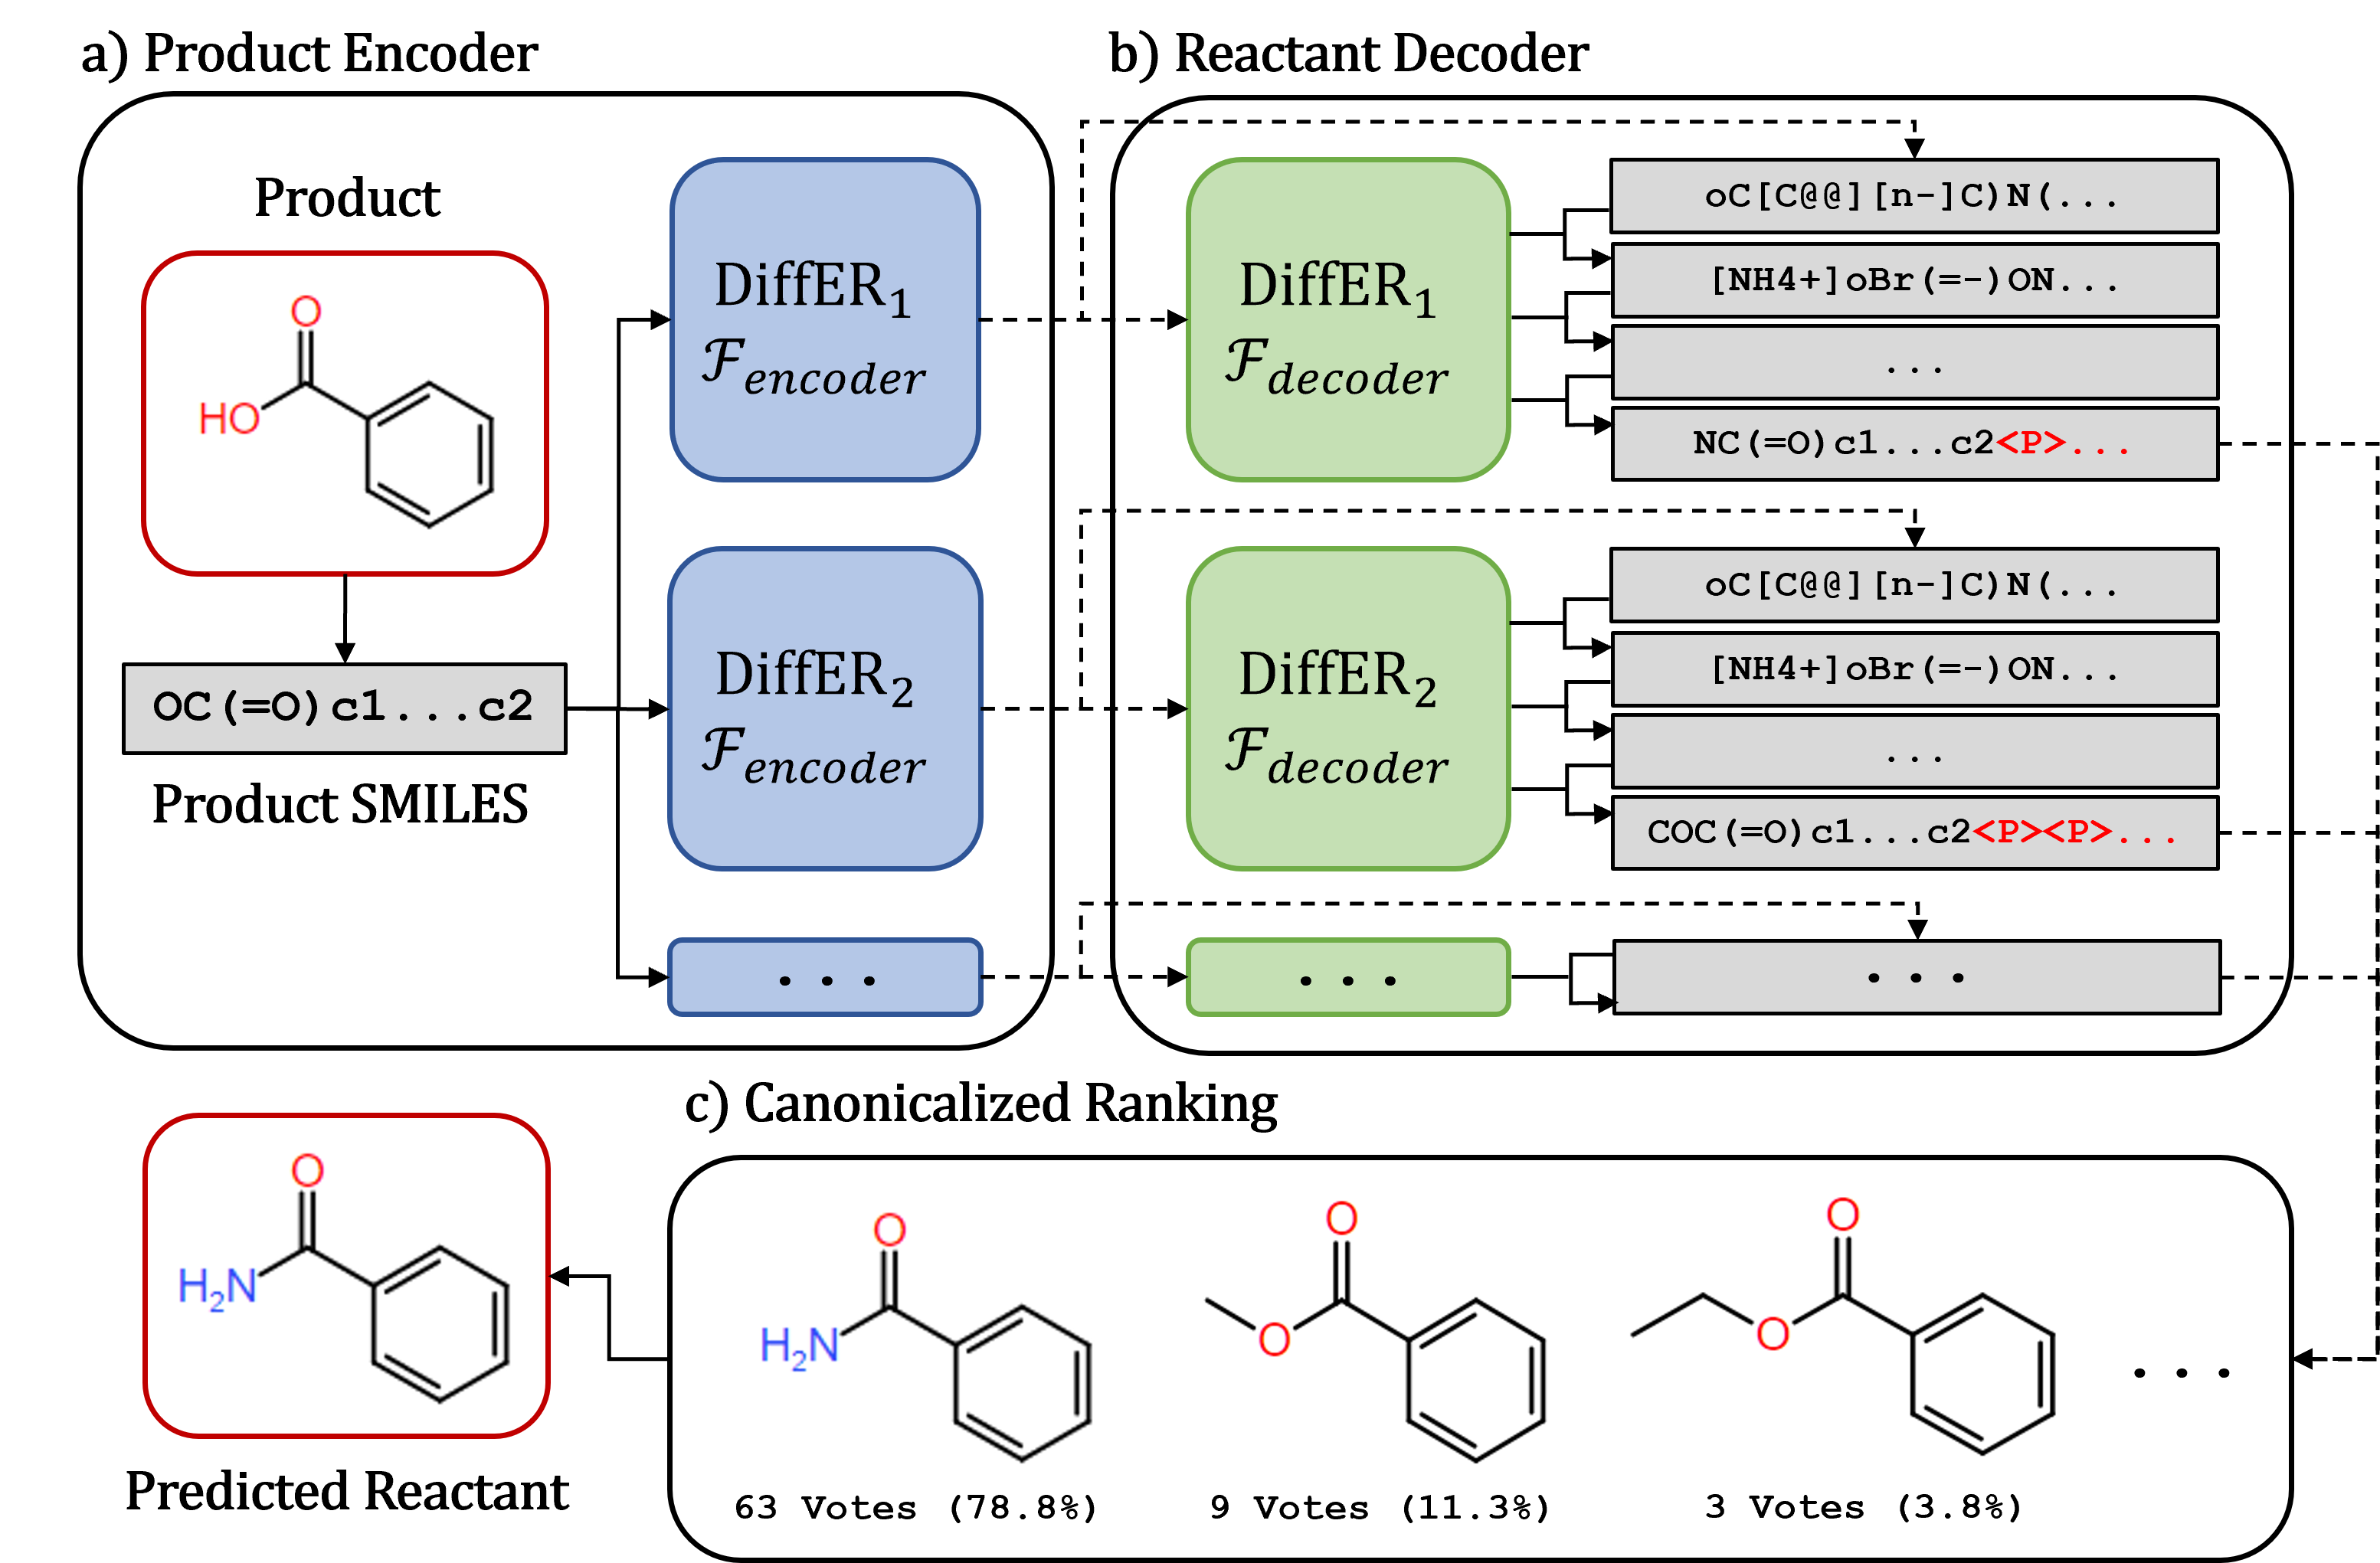
\includegraphics[width=0.9\linewidth]{images/diffusion_schema.png}
    \caption{Schematic of \ours, our diffusion process for retrosynthesis. \textbf{a)} The Product Encoder, which converts the product to a random, root-aligned SMILES form and encodes it using the encoder portion of the \ours models. The encoder models also predict the size of the diffusion noise vector. \textbf{b)} The Reactant Decoder, which diffuses the reactant from randomly initialized categorical noise using the decoder portion of the \ours models. Decoder models can predict pad tokens \texttt{<P>} to diffuse SMILES strings of varying lengths. \textbf{c)} The Canonicalized Ranking, which ranks the canonical molecules predicted by the \ours models by the number of times they are generated. The top-ranked reactant is the predicted reactant.}
    \label{fig:schema}
\end{figure}

\subsection{Methods}
\label{sec:methods}

% \subsection{Problem Setup}

We define the retrosynthesis task as a sequence-to-sequence modeling problem and combine the approaches of Hoogeboom et al. \cite{hoogeboom2021argmax}, DiffuSeq \cite{gong2022diffuseq, gong2023diffuseq}, and MaskPredict \cite{ghazvininejad2019mask} to train conditional, multinomial diffusion models for the retrosynthesis task. We utilize a traditional encoder-decoder transformer architecture to construct individual conditional diffusion models, where the encoder is responsible for learning the representation of the conditional features and the decoder acts as the diffusion approximation model. In the end, eight individual diffusion models are ensembled to produce \ours, a novel ensemble model for chemical retrosynthesis.

Let $\bm{x}_t \in \{0,1\}^{K \times \ell_x}$ be a sequence of $\ell_x$ one-hot encoded vectors of size $K$ representing the source and let $\bm{y}_t \in \{0,1\}^{K \times \ell_y}$ be similarly defined representing the target. Let $\mathcal{C}$ denote a categorical probability distribution with parametrized probability. Finally, let $\mathcal{F}$ represent a transformer neural network with encoder $\mathcal{F}_{\text{encoder}}$, decoder $\mathcal{F}_{\text{decoder}}$, and sequence length prediction classifier $\mathcal{F}_{\text{length}}$.

\subsubsection{Forward Noising Process}
Following Hoogeboom et al. \cite{hoogeboom2021argmax}, we define the multinomial diffusion process $q$ as a categorical distribution $\mathcal{C}$ with probability $\beta_t$ of sampling uniformly from $\{0, 1\}^K$ for any step in the sequence, and apply noising to the target matrix $y_t$:
\begin{equation}
    q(\bm{y}_t | \bm{y}_{t-1}) = \mathcal{C}(\bm{y}_t | (1-\beta_t)\bm{y}_{t-1} + \beta_t / K).
\end{equation}
This forms a Markov chain allowing $\bm{y}_t$ to be directly sampled from $\bm{y}_0$:
\begin{equation}
    q(\bm{y}_t | \bm{y}_0) = \mathcal{C}(\bm{y}_t | \bar{\alpha}_t\bm{y}_0 + (1 - \bar{\alpha}_t)/K),
\end{equation}
where $\alpha_t = 1 - \beta_t$ and $\bar{\alpha}_t = \prod_{\tau=1}^t\alpha_\tau$. Note that in the forward noising process, we only apply noise to the target sequence $\bm{y}_0$.

\subsubsection{Conditional Denoising}
We continue following the work of Hoogeboom et al. to denoise the categorical data. We construct the posterior distribution of the categorical model as
\begin{equation}
    p_{\theta}(\bm{y}_{t-1} | \bm{y}_t, \bm{y}_0) = \mathcal{C}(\bm{y}_{t-1} | \bm{\theta}_{\text{post}}(\bm{y}_t, \bm{y}_0)),
\end{equation}
where 
\begin{equation}
    \bm{\theta}_{\text{post}}(\bm{y}_t, \bm{y}_0) = \bar{\bm{\theta}}/\sum_{k=1}^K\hat{\theta}_k
\end{equation}
and
\begin{equation}
    \bar{\bm{\theta}} = [\alpha_t \bm{y}_t + (1 - \alpha_t)/K] \odot [\hat{\alpha}_{t-1} \bm{y}_0 + (1 - \hat{\alpha}_{t-1})/K].
\end{equation}

Notably, as $\bm{y}_0$ is not known during inference, it must be estimated using a neural network. Inspired by DiffuSeq \cite{gong2022diffuseq, gong2023diffuseq}, we concatenate a representation of the source sequence to the noised representation of the target sequence to use as input to the $\bm{y}_0$ approximation model. In contrast to DiffuSeq, which uses the embedded representation of the source sequence $\bm{x}_0$, we process the source sequence with a transformer encoder model prior to concatenating, which is used as the memory component in the decoder architecture \cite{lewis2019bart}. Thus, the reverse diffusion process is fully modeled as
\begin{equation}
    p_{\theta}(\bm{y}_{t-1} | \bm{y}_t, \bm{x}_0) = \mathcal{C}(\bm{y}_{t-1} | \bm{\theta}_{\text{post}}(\bm{y}_t, \mathcal{F}_{\text{decoder}}(\bm{y}_t || \mathcal{F}_{\text{encoder}}(\bm{x}_0)))),
\end{equation}
where $||$ is the concatenation operator. We denote the estimated target sequence as $\hat{\bm{y}}_0$. Additionally, we add a sinusoidal embedding of the current diffusion timestep $t$ to the diffusion model input $\bm{y}_{t}$.

\subsubsection{Length Prediction}
\label{sec:length_prediction}

One downside of the diffusion methodology compared to normal autoregressive methods is the requirement that the total length of the sequence must be known prior to inference so that the starting uniform noise distribution can be properly initialized. Prior work, such as DiffuSeq \cite{gong2022diffuseq, gong2023diffuseq}, have primarily approached this issue by padding the sequence with observable \texttt{PAD} tokens up to a maximum length, and allowing the diffusion model to predict the location of \texttt{PAD} tokens as necessary. In contrast, MaskPredict \cite{ghazvininejad2019mask} presents the idea of a length prediction token, which is learnt by the transformer encoder block and used to initialize the input to the transformer decoder. We similarly prepend a \texttt{LENGTH} token to the source sequence $\bm{x}_0$ and use the learned representation of the \texttt{LENGTH} token for the sequence to predict a target length $\hat{\ell}_y$:
\begin{equation}
    p(\hat{\ell}_y|\bm{x}_0) = \mathcal{F}_{\text{length}}(\mathcal{F}_\text{encoder}(\bm{x}_0)),
\end{equation}
where $\mathcal{F}_{\text{length}}$ is a feed-forward classifier function over integers up to the maximum sequence length dependent only on the first column of $\mathcal{F}_\text{encoder}(\bm{x}_0)$.

Upon initial testing, we find that the baseline implementation of MaskPredict length prediction performs poorly for this task due to its rigidity in predicting the sequence length and frequency of predicting shorter sequences than the ground truth. To remedy this, we propose a novel adjustment to the method by appending a uniform random number $n \sim \mathcal{U}(1, N)$ of observable padding tokens to the decoder sequences during training. This increases the expected length of the sequence by $\frac{(1 + N)}{2}$ while allowing the diffusion model to predict pad tokens within a range of the the target length. Notably, as the probability of predicting $n$ padding tokens is equivalent for $n \in [1, N]$, the probability of predicting sequences with lengths within $\frac{(1 + N)}{2}$ of the predicted length is approximately equal. This offers benefits of both the MaskPredict and DiffuSeq approaches: The diffusion model is provided with information about the target length from the encoder while still allowing for the possibility of predicting a variety of sequence lengths rather than only the predicted target length. Intuitively, lower limits of $N$ place more focus on the length prediction component, while higher values of $N$ allow the model to vary more from the initial length prediction. Additionally, as the lengths of the input source sequence and output target sequence of the retrosynthesis task are highly correlated, we shift the methodology to predict the difference in length between the source and target rather than the total length of the target.

\subsubsection{Ensemble Voting of Models}

In order to stabilize and diversify the output of the diffusion model, we implement an ensemble of various individual diffusion models with different values of the random padding limit $N$. During inference, multiple samples are drawn from each model trained on different $N$. Outputs are then ranked according to the number of times they are sampled overall. Ties are broken using a ranked-choice voting scheme. This process encourages output diversity by combining models trained with varying degrees of reliance on the length prediction component. We refer to the constructed ensemble model as \ours.

We identically construct and train the individual models that compose \ours,  varying only the maximum number of random padding that can be added on to the target sequence during training. We test various voting combinations of models with random padding limit $N \in \{5, 10, 15, 20, 30, 40, 50, 60, 70, 80, 90\}$. We find that models trained with $N < 20$ perform poorly, as they place too much focus on the length prediction component, which is biased toward a lower increase in length. We construct the final ensemble using eight models trained on $N \in \{20, 30, 40, 50, 60, 70, 80, 90\}$.

\subsubsection{Loss Functions}

We utilize a combination of mean square error (MSE) and variational lower bound (VLB) losses to train the diffusion models, the latter of which is derived using the Kullback-Leibler (KL) divergence according to Hoogeboom et al \cite{hoogeboom2021argmax}. We apply MSE loss directly to the predicted target $\bm{y}_0$, while the VLB loss uses the sampled posterior of the predicted target:
\begin{align}
    \mathcal{L}_{\text{MSE}} &= \mathbb{E}\left[||\bm{y}_0^2 - \hat{\bm{y}}_0^2||\right] \\
    \mathcal{L}_{\text{VLB}} &= \mathbb{E}\left[\sum_{k=0}^K\bm{y}_{0, k} \log \hat{\bm{y}}_{0, k} - \sum_{t=2}^T\text{KL}(q(\bm{y}_{t-1}| \bm{y}_t, \bm{y}_0) | q(\bm{y}_{t-1}| \bm{y}_t, \hat{\bm{y}}_0))\right].
\end{align}
Finally, we include a loss term for the length prediction task using cross entropy:
\begin{equation}
    \mathcal{L}_\ell = \mathbb{E}\left[\sum_{l=0}^L{\ell_y}_l\log p(\hat{\ell_y}|\bm{x}_0)_l\right],
\end{equation}
where $\ell_y$ is a one-hot encoded vector representing the length difference between $\bm{y}_{0}$ and $\bm{x}_0$. Additionally, when training the diffusion models, we employ the importance-based time sampling algorithm used in DiffuSeq \cite{gong2022diffuseq, gong2023diffuseq}.

\subsubsection{Reproducibility}

We apply our models to the USPTO-50K \cite{Lowe2017} data set with Root-aligned SMILES augmentation \cite{zhong2022root}, which greatly improves the performance of the diffusion models. We directly utilize the dataset splits provided by the authors of Root-aligned SMILES. We form \ours as an ensemble of models with random padding limit $N \in \{20, 30, 40, 50, 60, 70, 80, 90\}$. Each model takes the form of a encoder-decoder transformer architecture with 6 layers and 8 attention heads with hidden dimension size 512, feed-forward size 2048, and GELU activation \cite{hendrycks2016gaussian}. We utilize an Adam optimizer with learning rate $1\times 10^{-4}$ and dropout rate of $0.1$. We set the number of diffusion steps to $T=200$. We use a cosine beta schedule \cite{chen2023importance} and a Gumbel-softmax distribution for noise sampling during the diffusion process. All models are trained using a high-performance computer with Intel Xeon E5-2680 v4 CPUs (128GB memory) and NVIDIA Tesla P100 GPUs (16GB memory).

During inference, we follow the work of Zhong et al. \cite{zhong2022root} to augment the input SMILES strings. 20 random Root-aligned SMILES strings are generated for each input product and provided to \ours for sampling. Thus, each model in \ours outputs 20 random samples for the input string. Output samples are canonized and ranked according to rate of occurrence.

\section{Results}
\label{sec:results}

\begin{table}[h!]
    \small
    \centering
    \caption{Top-K accuracy for tempate-based, semi-template, and template-free retrosynthesis models. The best performing model of its category for each $K$ is 
    in \textbf{bold} and the second best model is \underline{underlined}. \ours is the best performing model for $K=1$ and the second best model for $K=3,5$ among template-free methods.}
    \begin{tabular}{l l r r r r}
        \toprule
         Category & Model & K=1 & 3 & 5 & 10 \\
        \midrule
        \multirow{4}{*}{Template-based} & Retrosim \cite{coley2017computer} & 37.3 & 54.7 & 63.3 & 74.1 \\
                                           & Neuralsym \cite{segler2017neural} & 44.4 & 65.3 & 72.4 & 78.9 \\
                                           & GLN \cite{dai2019retrosynthesis} & \underline{52.5} & \underline{69.0} & \underline{75.6} & \underline{83.7} \\
                                           & LocalRetro \cite{chen2021deep} & \textbf{53.4} & \textbf{77.5} & \textbf{85.9} & \textbf{92.4} \\
        \midrule
        \multirow{5}{*}{Semi-template} & G2Gs \cite{shi2020graph} & 48.9 & 67.6 & 72.5 & 75.5 \\
                                          & GraphRetro \cite{somnath2021learning} & \underline{53.7} & 68.3 & 72.2 & 75.5 \\
                                          & RetroXpert \cite{yan2020retroxpert} & 50.4 & 61.1 & 62.3 & 63.4 \\
                                          & RetroPrime \cite{wang2021retroprime} & 51.4 & \underline{70.8} & \underline{74.0} & \underline{76.1} \\
                                          & G$^2$Retro \cite{chen2023g} & \textbf{53.9} & \textbf{74.6} & \textbf{80.7} & \textbf{86.6} \\
        \midrule
        \multirow{11}{*}{Template-free} & Seq2Seq \cite{liu2017retrosynthetic} & 37.4 & 52.4 & 57.0 & 61.7 \\
                                          & Levenshtein \cite{sumner2020levenshtein} & 41.5 & 48.1 & 50.0 & 51.4 \\
                                          & GTA \cite{seo2021gta} & 51.1 & 67.6 & 74.8 & 81.6 \\
                                          & Graph2SMILES \cite{tu2022permutation} & 51.2 & 66.3 & 70.4 & 73.9 \\
                                          & Dual-TF \cite{sun2021towards} & 53.3 & 69.7 & 73.0 & 75.0 \\
                                          & MEGAN \cite{sacha2021molecule} & 48.1 & 70.7 & 78.4 & 86.1 \\
                                          & Chemformer \cite{irwin2022chemformer} & 54.3 & - & 62.3 & 63.0 \\
                                          & Retroformer \cite{wan2022retroformer} & 53.2 & 71.1 & 76.6 & 82.1 \\
                                          & Tied transformer \cite{kim2021valid} & 47.1 & 67.2 & 73.5 & 78.5 \\
                                          & R-SMILES \cite{zhong2022root} & \underline{56.3} & \textbf{79.2} & \textbf{86.2} & \textbf{91.0} \\
        \cmidrule(lr){2-6}                                   
                                          & \ours & \textbf{57.6} & \underline{79.0} & \underline{84.1} & \underline{87.4} \\
        \midrule
                                           
    \end{tabular}
    \label{tab:topk}
\end{table}

We compare \ours to a variety of template-based, semi-template, and template-free methods for retrosynthesis prediction with unknown reaction types, detailed in Appendix \ref{sec:A1}. We report top-k accuracy for $k\in\{1,3,5,10\}$ following standard procedures. We construct \ours as an ensemble of eight diffusion models with various hyperparameters and sample from each model twenty times with augmented input SMILES according to the work of Zhong et al. \cite{zhong2022root}. Predicted reactants sampled from the diffusion models are ranked according to the number of times they were predicted by the diffusion models. By using multiple different models with different hyperparameters to predict possible reactants for the same reaction, we encourage diversity and stability in the output reactants. Ties in reactant rankings are decided according to a ranked choice voting scheme. Further ties are broken arbitrarily. Results for the diffusion ensemble model are reported against baseline algorithms in Table \ref{tab:topk}.
%, while individual model results are reported in Table \ref{tab:indv_models} in appendix \ref{sec:A2}. We include a short review of the baselines used for comparison in appendix \ref{sec:A1}.

Notably, \ours is the best performing model for $K=1$ (57.6\%) across all model types, and is highly competitive for higher values of $K$, achieving the second best performance for $K=3$ (79.0\%) behind Root-Aligned SMILES \cite{zhong2022root} and third best performance for $K=5$ and $K=10$ (84.1\% and 87.4\%, respectively) behind Root-aligned SMILES and LocalRetro \cite{chen2021deep}, making it the second best model among template-free approaches. The decrease in performance of ours at higher values of $K$ can likely be attributed to a lack of outputs for higher values of $K$: despite generating outputs from multiple models for a diversity of input product SMILES, the output of \ours tends to produce just a few candidate reactant sets for each product, producing the same output molecule numerous times in a different, non-canonical SMILES form. Indeed, Figure \ref{fig:num_samples} shows a histogram of the number of sample reactions generated for the test dataset. The diffusion ensemble produces a median number of samples of 9, with 17.9\% of reactions producing less than 5 samples, and 57.1\% producing less than 10. Notably, we find that fewer reactants tend to be sampled when \ours is correct in its output: reactions where the top-1 reactant is correctly predicted produce only 8.4 different molecules on average, compared to 12.3 for cases where the top-1 reactant does not match the ground truth. This lack of outputs is less observed in other methods such as R-SMILES which apply beam-search algorithms to sequential decoders, allowing a greater number of possible reactants to be found. 

\begin{figure}[h]
    \small
    \centering
    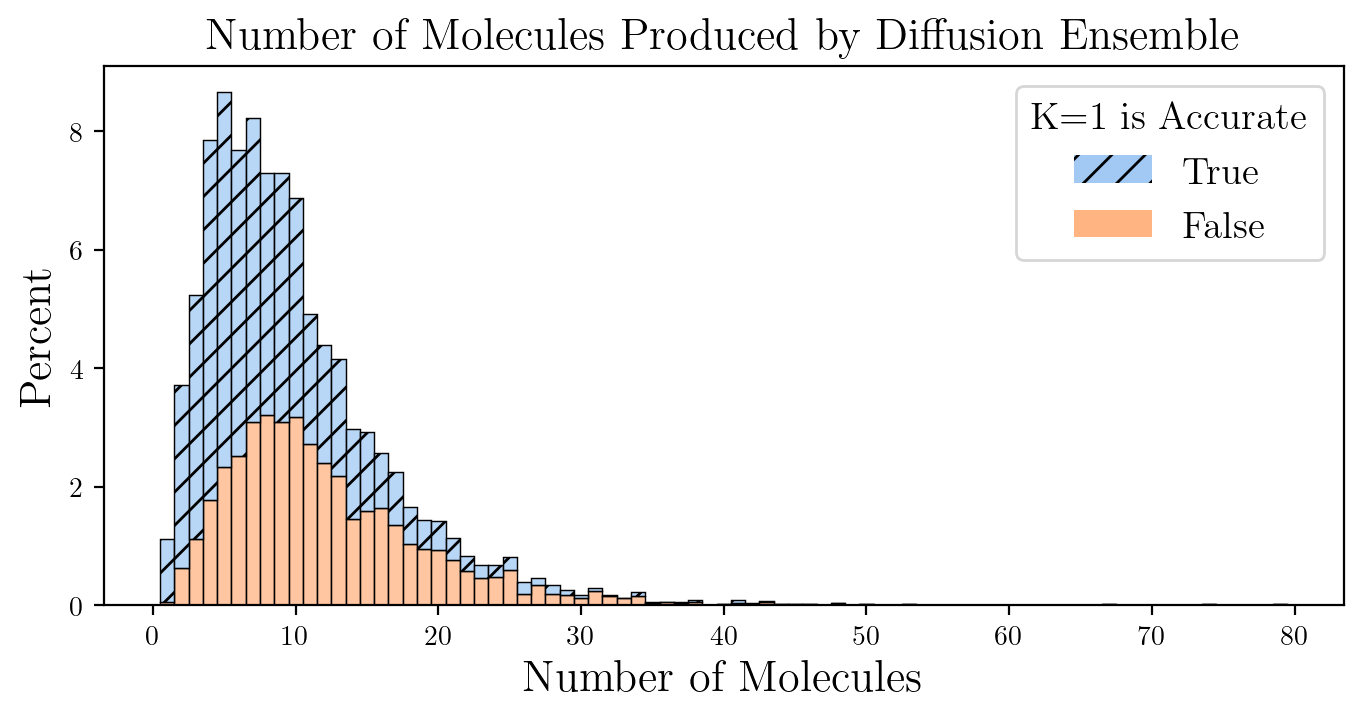
\includegraphics[width=0.7\linewidth]{images/num_samples_histogram.png}
    \caption{A histogram of the number of different molecules output by \ours for each reaction during inference.The distribution has a mean of 10.0 and a median of 9. ``K=1 is Accurate'' indicates if the most commonly predicted molecule matched the ground-truth reaction.}
    \label{fig:num_samples}
\end{figure}

\subsection{Individual Model Performance}

We construct \ours from eight individually trained diffusion models, each of which uses a different random padding limit $N$ (described in Section \ref{sec:length_prediction}) during training. We report the individual performance for each of the trained models in Table \ref{tab:our_models}. We compare these results to the \ours ensemble as well as a baseline diffusion model trained using direct length prediction, without the length variation used in the individual \ours models, also reported in Table \ref{tab:our_models}.

The individual \ours models greatly improve upon the baseline length prediction model, demonstrating the effectiveness of our length variation technique. The length variation technique encourages the individual models to over-predict the length of the reactant SMILES and then reduce the output SMILES to the correct size using predictable padding tokens. Meanwhile, the baseline length prediction model drastically under-performs all other models in terms of accuracy, demonstrating the sensitivity of the diffusion models for SMILES string generation to the size of the noise vector. Both the individual \ours models and the baseline length prediction model exhibit low variance in the output reactants, only predicting 3.2 and 3.8 reactants on average, respectively. Notably, all models still achieves high validity from among the output molecules, indicating that the individual diffusion models are properly learning not only the SMILES grammar, but also rules of molecular validity.

When the individual models are ensembled into the complete \ours model, both the accuracy and diversity of predicted reactants are significantly improved. The \ours ensemble produces on average twice the number of reactants compared to the individual models, highlighting the impact of the different individual model setups on the output molecules. By combining multiple models trained on different upper limits for the length of the SMILES string, we can leverage different weightings of the length prediction mechanism. When a model is trained on a lower padding limit, more emphasis is placed on the length prediction component, as the model is less able to diverge from the predicted length. When the padding limit is larger, the diffusion model has more freedom to construct SMILES of varying lengths, but are less informed by the length prediction. By combining multiple models on various random padding limits, we improve the diversity and accuracy of the predicted reactants.

\begin{table}[h]
    \small
    \centering
    \caption{Comparison of the \ours ensemble with the individual models that make up \ours. Individual models are notated as \ours$_N$, where $N$ represents the upper bound on the number of added padding tokens according to the procedure in Section \ref{sec:length_prediction}. We additionally include single models with baseline length prediction and oracle length prediction. The individual \ours models show significantly higher accuracy than baseline length prediction, but are outperformed by the \ours ensemble. The oracle length model drastically outperforms all existing models.}
    \begin{tabular}{r r r r r r r}
        \toprule
        Model & K=1 & 3 & 5 & 10 & Sample Validity & Avg. Num. Reactants \\
        \midrule
        \ours Ensemble & 57.6 & 79.0 & 84.1 & 87.4 & 100.0 & 10.0 \\
        \midrule
        \ours$_{20}$ & 53.2 & 70.3 & 72.9 & 73.6 & 100.0 & 3.2 \\
        \ours$_{30}$ & 55.2 & 71.5 & 74.4 & 75.2 & 99.9 & 3.2 \\
        \ours$_{40}$ & 54.6 & 72.1 & 74.4 & 75.3 & 99.9 & 3.2 \\
        \ours$_{50}$ & 54.9 & 71.3 & 73.7 & 74.4 & 100.0 & 3.2 \\
        \ours$_{60}$ & 55.4 & 71.7 & 74.6 & 75.4 & 99.9 & 3.3 \\
        \ours$_{70}$ & 54.3 & 71.1 & 73.5 & 74.4 & 99.6 & 3.2 \\
        \ours$_{80}$ & 54.6 & 71.9 & 74.4 & 75.1 & 99.6 & 3.3 \\
        \ours$_{90}$ & 54.5 & 71.6 & 74.2 & 74.9 & 99.8 & 3.3 \\
        \midrule
        Baseline Length & 40.4 & 55.9 & 58.8 & 59.9 & 99.9 & 3.8 \\
        Oracle Length & 77.0 & 88.1 & 89.5 & 90.0 & 99.7 & 2.8 \\
        \midrule
    \end{tabular}
    \label{tab:our_models}
\end{table}

\paragraph{Upper Limits on Performance}
we additionally consider a upper limit on the performance of categorical diffusion models for chemical retrosynthesis by considering an oracle model which predicts the length of the output SMILES string with 100\% accuracy. This allows us to construct a diffusion model without needing to incorporate aspects of length prediction or variability in the size of the output as discussed in Section \ref{sec:length_prediction}. Under the assumption of the length-predicting oracle, we can initialize input noise to the diffusion model of the proper size. We run this experiment for a single diffusion model and utilize the same parameters and repeated sampling during inference as discussed in the experimental setup.

Results for this experiment are presented in Table \ref{tab:our_models} in comparison to the \ours models and the baseline length prediction diffusion model. The model with oracle length drastically outperforms \ours as well as all existing methods for $K=1,3,5$, but performs slightly worse than both Root-aligned SMILES and LocalRetro for $K=10$. Similarly to \ours, this can be attributed to a lack of variety in the predicted output, which is even more extreme for the oracle length model: on average, only 2.8 different reactants are predicted, with a median of just 2 predicted reactants. However, this lack of diversity is overcome by the oracle model's high accuracy amongst the predicted reactants.

This result highlights the importance of accurate length prediction in non-auto-regressive models, particularly in the case of molecular generation with SMILES strings. While there is some variability in the length of randomly generated SMILES string for a specific molecule, these variants generally only differ by a length of two or three, if they differ at all. If the length prediction is off from a viable value by even one or two, it may force an entirely different molecule to be generated, resulting in lower reported performance. By including the random length padding in \ours, we help combat the diffusion model's sensitivity to length prediction, but remain far from the performance of a model with perfect length prediction.

\section{Discussion}
\label{sec:discussion}

Our results show that categorical diffusion models offer a competitive alternative to auto-regressive models for template-free single step retrosynthesis prediction and are able to outperform state-of-the-art template-based, semi-template, and template-free methods on top-1 accuracy, and achieve similar performance to state-of-the-art models on top-3, top-5, and top-10 accuracy. The proposed \ours ensemble is able to efficiently sample from the posterior distribution of possible reactant SMILES strings while maintaining the viability of output SMILES. \ours is capable of reproducing existing patented reactions as well as proposing new and viable reactants (Appendix \ref{sec:case_study}).

% \subsection{Comparison to Other Template-free Methods}

% Compared to other template-free methods, our diffusion ensemble is able to construct the entire reactant SMILES string in unison, rather than token by token. Methods like Chemformer \cite{irwin2022chemformer} or R-SMILES \cite{zhong2022root} build the SMILES sequence by predicting a distribution of probabilities for the next token conditioned on the current sequence and then selecting the token with the highest probability and adding it to the sequence. To generate multiple possible reactants, auto-regressive methods generally use beam-search algorithms to generate multiple possible reactants \cite{irwin2022chemformer}. Beam-search algorithms explore multiple options at each step, and only continue exploring the top-k sequences with the highest probability. In contrast, our diffusion approach directly samples an entire reactant SMILES string from the approximated posterior distribution of possible reactants. Thus, the proportion of times a molecule is sampled from \ours can be interpreted as a approximation of the posterior probability of that reactant. This offers an interpretable measure of confidence in the model outputs. However, this form of sampling also results in limited diversity in the output reactant set: when the model is highly confident or little diversity exists in the space of possible reactants, only a few possible reactants may be produced. In contrast, when the model is unsure or there is a high number of possible reactions, more reactants will be produced. This trade-off can be disadvantageous in certain circumstances, particularly when there is a low number of predicted reactants and the top-predicted reactant is unsuitable.

% \subsection{Comparison to Template-based and Semi-template Methods}

% Unlike template-based and semi-template methods, diffusion models do not directly utilize a static set of reaction templates. Rather, \ours learn suitable reactions directly from the data, allowing for greater generalization to reactions that may occur outside the realm of existing templates. However, this comes at a notable cost in interpretability: because the diffusion method constructs the proposed reactants from randomly generated uniform noise, it is not always clear what causes the emergence of a particular reactant over another possible reactant. A greater analysis of the latent noise would need to be done to further understand the workings of \ours. In contrast, template-based and semi-template based methods directly utilize the existing molecular structure and set of reaction templates when determining where reaction centers are and which reaction templates apply. This offers a greater level of interpretability and scientific backing than template-free methods.

\subsection{Limitations and Directions of Future Work}

Despite the strong performance of \ours, there are a few notable limitations to the modeling approach. Firstly, raw diffusion models are highly sensitive to the predicted size of the output. Thus, methods such as our novel variant length padding (Section \ref{sec:length_prediction}) must be employed to diversify target lengths and allow diffusion models to predict molecules of varying size. Secondly, \ours suffers from a lack of output variety, often producing just a few possible reactants. Because diffusion models sample from an approximated posterior, reactants which the model deems more probable will be sampled at a higher rate, resulting in fewer reactants being sampled overall for a static sample size. This is particularly true in cases where the model is confident in its prediction. Finally, the model sometimes produces sub-optimal reactions, such as some of those displayed in Appendix \ref{sec:case_study}. Such reactions often undergo additional reactions alongside the target reaction, and while the desired product is a possible outcome, additional byproducts would likely be produced in many cases. These limitations highlight necessary areas of future research for not only categorical diffusion models in chemical retrosynthesis, but also categorical diffusion models for sequence generation in general:
\begin{enumerate}
    \item Categorical diffusion models must be able to adapt to differently sized outputs. Prior work relies on predictable padding tokens to predict differently sized sequences \cite{gong2022diffuseq, gong2023diffuseq}, but this reliance can introduce its own biases due to the prevalence of padding tokens for shorter sequences. \ours overcomes reliance on predicting padding tokens by adding limited variability in the number of possible padding tokens, with some success; however, results still pale in comparison to a model with perfect sequence length prediction.
    \item Additional techniques to sample categorical diffusion models must be developed in order to improve sequence diversity and coverage. Compared to the traditional applications of diffusion models in image generation, molecular SMILES generation has significantly fewer possible outputs, making the models more likely to converge to a single prediction. This effect is heightened by the the presence of multiple SMILES strings mapping to the same molecular structure: while the sequence itself may be different, the same molecule is produced. We must develop methods to encourage greater output diversity in the sampled molecules. \ours attempts encourages output diversity using an ensemble approach, and while the results are significantly more diverse than single model approaches, the number of differently sampled molecules remains low.
\end{enumerate}
The case studies of \ours presented in Appendix \ref{sec:case_study} additionally demonstrate directions of future research for retrosynthetic modeling as a whole, many of which are echoed in other work \cite{chen2023g}:
\begin{enumerate}
    \setcounter{enumi}{2}
    \item Machine learning models for retrosynthesis are generally unaware of possible side products as a result of the generally available training data. Because these models are most commonly trained on patent reaction datasets, models are not generally exposed to explicit examples where multiple possible outcomes could occur. Indeed, the UPSTO-50K dataset has no reactant sets which map to more than one molecule, limiting the ability of the model to learn that multiple reactions may be possible for a single set of reactants. To improve the ability of ML models to understand chemical processes, incorporating additional examples into the training datasets may be beneficial, and with proper learning techniques, may lead to improved performance.
    \item Evaluating the performance of ML models on chemical retrosynthesis most commonly relies on a) matching to patented reactions and b) analyzing individual case studies. Evaluating models by matching to patented reactions limits the discovery of novel techniques and pathways, as models may produce valid results that do not match patent data. In contrast, evaluating individual case studies is more adaptable to understanding the model's true performance, but is a time consuming process requiring considerable chemical knowledge. To enhance the development of ML models for chemical retrosynthesis, we must develop new methods of analysis that take into account the abundance of viable reactions as well as existing chemical knowledge.
\end{enumerate}
Further research in these four tasks would greatly benefit the application of diffusion models in chemical retrosynthesis, as well as both diffusion modeling and retrosynthetic prediction models individually.


\section{Conclusion}

Our ensemble of categorical diffusion models provides state-of-the-art top-1 accuracy as well as competitive top-3 and top-5 accuracy.
% We demonstrate that our ensemble model is capable of not only reproducing patented reactions, but also producing viable alternative reactions for the same product. 
Additionally, we offer insight into the importance of length prediction and length variation methods when training diffusion models for sequence prediction tasks.
% Finally, we include an analysis and discussion of the limitations of our approach.
We hope this work provides a suitable baseline and opens new avenues of exploration for a new class of template-free retrosynthesis model which differs from current autoregressive approaches. In future work, we plan to investigate additional methods of length prediction, as well as apply different diffusion sampling techniques to improve the diversity of sampled molecules. Finally, we plan to continue improving upon the diffusion model that comprise \ours, introducing methods such as adaptive noise scheduling \cite{yuan2022seqdiffuseq} as well as other advancements in categorical diffusion models to improve model performance.

\begin{ack}
This project was made possible, in part, by support from the National Science Foundation grant no. IIS-2133650 and the National Library of Medicine grant no. 1R01LM014385. Any opinions, findings and conclusions or recommendations expressed in this paper are those of the authors and do not necessarily reflect the views of the funding agency.
\end{ack}

\bibliographystyle{plain}
\bibliography{references}


\small



%%%%%%%%%%%%%%%%%%%%%%%%%%%%%%%%%%%%%%%%%%%%%%%%%%%%%%%%%%%%

\appendix

\section{Appendix / supplemental material}


\subsection{Case Studies}
\label{sec:case_study}


We offer additional results in the form of a case study of four different reactions, the results of which can be seen in Figures \ref{fig:case_study1} and \ref{fig:case_study2}. We select four different reactions from the test dataset to highlight the successes and limitations of the diffusion models. For each reaction, we report the top-3 reactants sampled from the diffusion ensemble.

\begin{figure}[!b]
    \footnotesize
    \centering
    \begin{tabular}{c c c c c}
    % \midrule
        \multirow{2}{*}{\textbf{a)}} &
        %CC(C)(C)OC(=O)c1c(N)ccc2c1OCC3C2(C3)
        \subf{\raisebox{0.3\height}{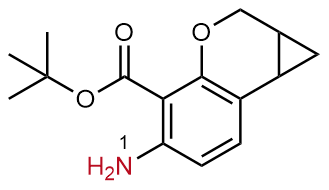
\includegraphics[width=0.15\linewidth]{images/molecules/case11_source.png}}}{\textbf{3aa}, desired product} & 
        \subf{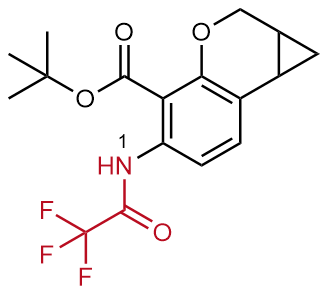
\includegraphics[width=0.15\linewidth]{images/molecules/case11_target.png}}{\textbf{3ab}, ground-truth reactants} & \\ &
        \subf{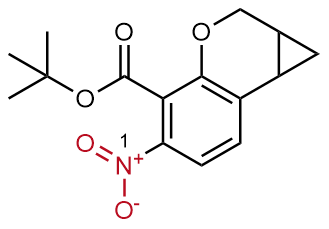
\includegraphics[width=0.15\linewidth]{images/molecules/case11_rank1.png}}{\textbf{3ac}, top-1 reactants (89.4\%)} & 
        \subf{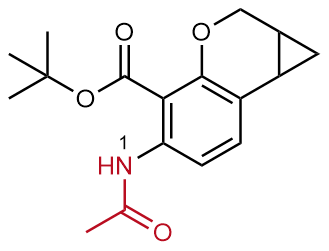
\includegraphics[width=0.15\linewidth]{images/molecules/case11_rank2.png}}{\textbf{3ad}, top-2 reactants (3.0\%)} & 
        \subf{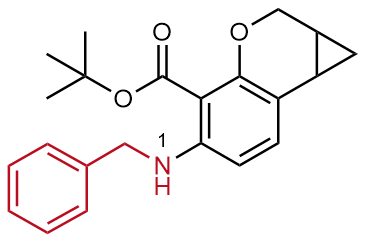
\includegraphics[width=0.15\linewidth]{images/molecules/case11_rank3.png}}{\textbf{3ae}, top-3 reactants (1.5\%)} \\
        \\
        \multirow{2}{*}{\textbf{b)}} &
        %CC(O)c1cccc(c1)C(=O)NC1=C(C(=O)N)Oc2ccc(F)cc21
        \subf{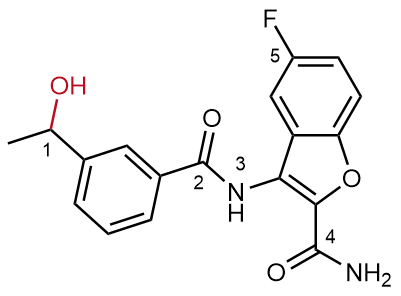
\includegraphics[width=0.18\linewidth]{images/molecules/case12_source.png}}{\textbf{3ba}, desired product} & 
        \subf{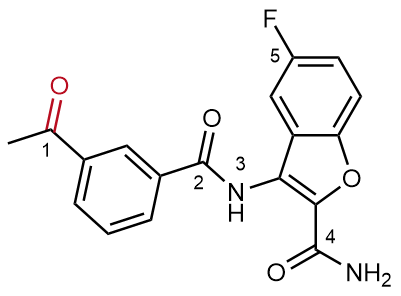
\includegraphics[width=0.18\linewidth]{images/molecules/case12_target.png}}{\textbf{3bb}, ground-truth reactants} & \\ &
        \subf{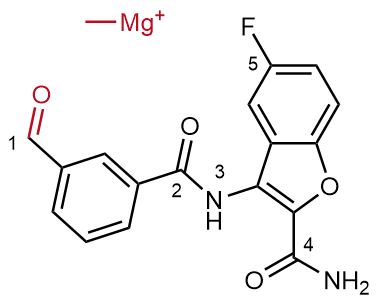
\includegraphics[width=0.18\linewidth]{images/molecules/case12_rank1.png}}{\textbf{3bc}, top-1 reactants (42.2\%)} & 
        \subf{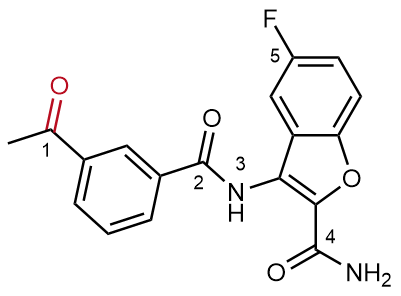
\includegraphics[width=0.18\linewidth]{images/molecules/case12_target.png}}{\textbf{3bd}, top-2 reactants (38.3\%)} & 
        \subf{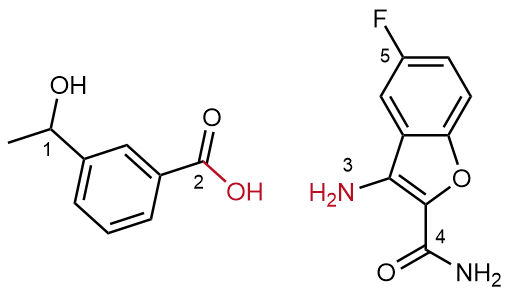
\includegraphics[width=0.24\linewidth]{images/molecules/case12_rank3.png}}{\textbf{3be}, top-3 reactants (9.7\%)} \\
    \end{tabular}
    \caption{Top-3 reactants for target products \textbf{a} and \textbf{b}from the test set compared to patent reactants. Values in parentheses indicated the percentage of time that reactant was sampled from the diffusion models. Numbers next to atoms are labels used to refer to the atom. Colored regions indicate where in the molecule a reaction is expected to occur.}
    \label{fig:case_study1}
\end{figure}

Reaction \textbf{a} (Fig. \ref{fig:case_study1}a) is a deprotection reaction in the forward direction in which the trifluoroacetamide protecting group (Fig. \ref{fig:case_study1}ab) is reacted with sodium borohydride in an ethanol solution to produce a primary amine at at the N1 position (Fig. \ref{fig:case_study1}aa). The diffusion ensemble does not predict this reactant, however, instead opting for the reduction of a nitro group, predicted 89.4\% of the time, (Fig. \ref{fig:case_study1}ac) at the N1 position. This is a widely used and viable reaction involving metal catalyzed reduction of the nitro group using Fe, Zn, Pd or Ni. Similarly, the third ranked choice (Fig. \ref{fig:case_study1}ae) is also a viable option involving a debenzylation reaction which is commonly performed in the presence of a metal catalyst under a hydrogen atmosphere. The second choice reaction (Fig. \ref{fig:case_study1}ad), however, undergoes amide hydrolysis under harsh conditions such as a strong acid. While this is also a viable synthesis, a harsh condition such as a strong acid would likely interact with the tert-butyl ester group leading to unwanted side products. Notably, the diffusion ensemble does not predict the patented reactant, primarily predicting the reduction of a nitro group 89.4\% of the time. We hypothesize that this is a result of the specific use-case of the ground-truth reaction, which is likely used in an industrial setting. Unlike the top-1 (Fig. \ref{fig:case_study1}ac) reactant, the ground-truth (Fig. \ref{fig:case_study1}ab) does not use the metal catalyzed reduction of a nitro group (top-1) or debenzylation (top-3) under a hydrogen atmosphere because it is not a safe reaction on industrial scale. While the top-1 or top-3 reactants may actually be more common in an academic lab setting, the ground-truth reactant is likely preferable on a large-scale industrial setting.

Reaction \textbf{b} (Fig. \ref{fig:case_study1}b) is a common reduction reaction of a ketone at C1 (Fig. \ref{fig:case_study1}bb) with sodium borohydride in a methanol solution to produce a secondary alcohol (Fig. \ref{fig:case_study1}ba). This same reaction is also predicted by the diffusion models 38.3\% of the time to give the second most popular predicted reactants (Fig. \ref{fig:case_study1}bd). The most popular predicted reactants  is an aldehyde and  Grignard reagent, predicted 42.2\% of the time, in which the methylmagnesium bromide reacts with the aldehyde at position C1 (Fig. \ref{fig:case_study1}bc) to produce the desired product in the forward reaction. However, the Grignard reagent (MeMgBr), which is a more nucleophilic reagent, is likely to react with other functional groups present in the molecule as well, such as the two amides at C2 and C4 or displace the fluorine at C5 via a nucleophilic aromatic substitution-like type reaction. In contrast, while the ground-truth/second-most predicted reaction (Fig. \ref{fig:case_study1}bb/\ref{fig:case_study1}bd) could lead to unwanted products, such as the reduction the carbonyl groups at C2 and C4, these reactions are less likely to occur compared to the Grignard reaction under a proper choice of reagents such as sodium borohydride in ethanol. The top-3 reactant is predicted just 9.7\% of the time, and unlike the other proposed reactants, it does not interact with the C1 carbon. Instead, it disconnects the molecule at the C1-N3 amide to reveal a C1 carboxylic acid and an N3 amine (Fig. \ref{fig:case_study1}be). The amide bond can be constructed in the forward reaction using a suitable amide coupling reaction condition. Yet again, this reaction is viable but would likely produce unwanted byproducts if other functional groups such as the free secondary alcohol or the primary amide in the proposed reaction were not protected first.

\begin{figure}[!b]
    \footnotesize
    \centering
    \begin{tabular}{c c c c c}        
        \multirow{2}{*}{\textbf{c)}} &
        %Fc1ccc(cc1)COc1ccc(C)cc1C1=CC=C(C)N1c1cc(C(O)=O)cc(c1)N1CCCC1(=O)
        \subf{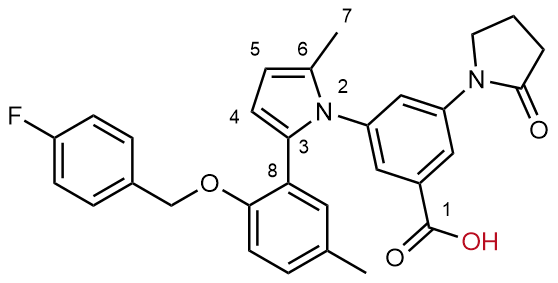
\includegraphics[width=0.24\linewidth]{images/molecules/case17_source.png}}{\textbf{3ca}, desired product} & 
        \subf{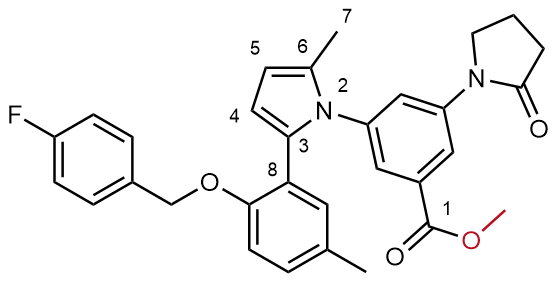
\includegraphics[width=0.24\linewidth]{images/molecules/case17_target.png}}{\textbf{3cb}, ground-truth reactants} & \\ &
        \subf{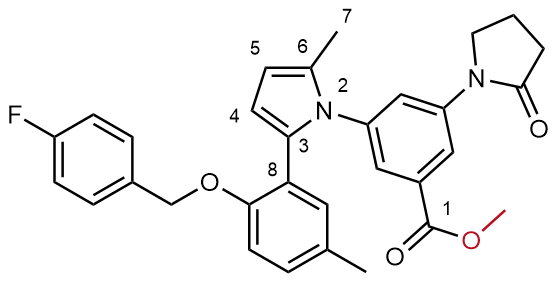
\includegraphics[width=0.24\linewidth]{images/molecules/case17_target.png}}{\textbf{3cc}, top-1 reactants (61.3\%)} & 
        \subf{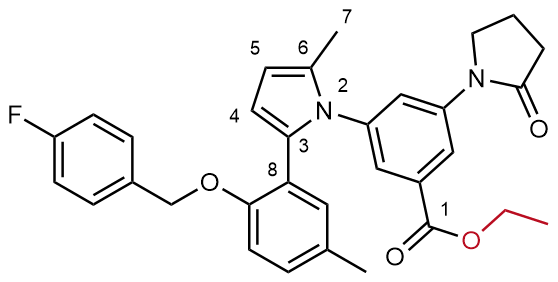
\includegraphics[width=0.24\linewidth]{images/molecules/case17_rank3.png}}{\textbf{3cd}, top-2 reactants (18.7\%)} & 
        \subf{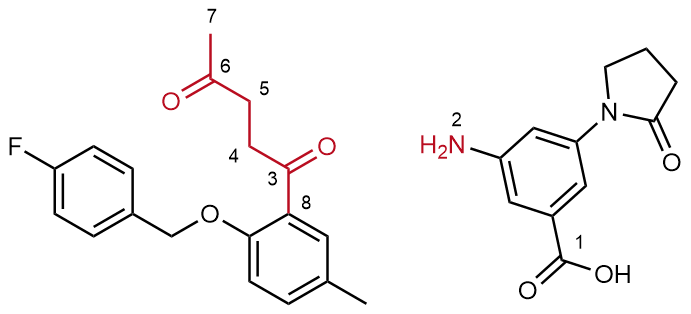
\includegraphics[width=0.29\linewidth]{images/molecules/case17_rank2.png}}{\textbf{3ce}, top-3 reactants (16.7\%)} \\
        \multirow{2}{*}{\textbf{d)}} &
        %COc4cccc5OCC(N(CCCCc1c[nH]c2ccc(F)cc12)C3CCC3)Cc45
        \subf{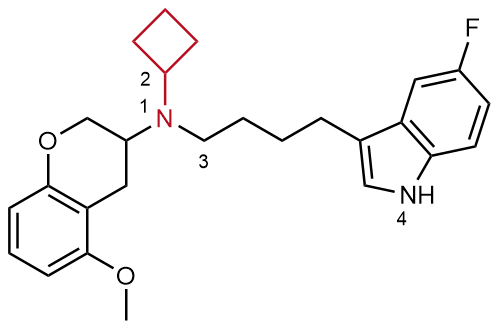
\includegraphics[width=0.2\linewidth]{images/molecules/case18_source.png}}{\textbf{3da}, desired product} & 
        \subf{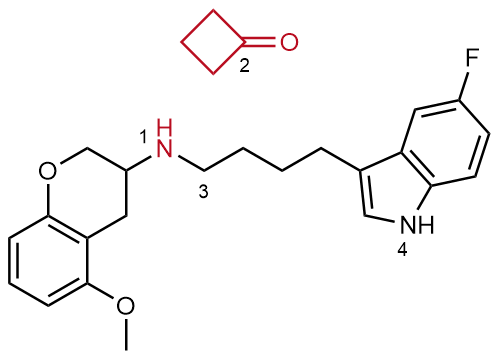
\includegraphics[width=0.2\linewidth]{images/molecules/case18_target.png}}{\textbf{3db}, ground-truth reactants} & \\ &
        \subf{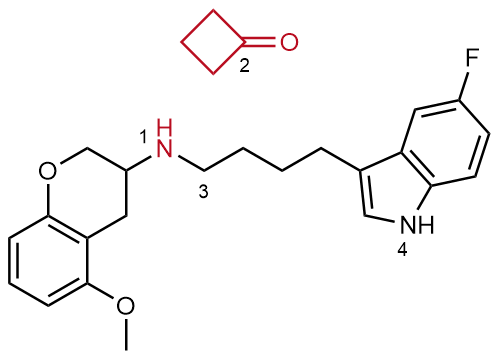
\includegraphics[width=0.2\linewidth]{images/molecules/case18_target.png}}{\textbf{3dc}, top-1 reactants (74.3\%)} & 
        \subf{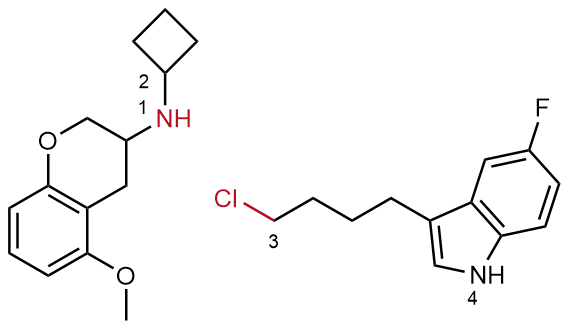
\includegraphics[width=0.24\linewidth]{images/molecules/case18_rank2.png}}{\textbf{3dd}, top-2 reactants (11.5\%)} & 
        \subf{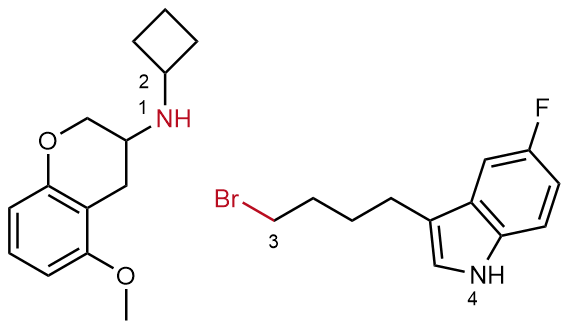
\includegraphics[width=0.24\linewidth]{images/molecules/case18_rank3.png}}{\textbf{3de}, top-3 reactants (2.7\%)} \\
    \end{tabular}
    \caption{Top-3 reactants for target products \textbf{c} and \textbf{d}from the test set compared to patent reactants. Values in parentheses indicated the percentage of time that reactant was sampled from the diffusion models. Numbers next to atoms are labels used to refer to the atom. Colored regions indicate where in the molecule a reaction is expected to occur.}
    \label{fig:case_study2}
\end{figure}

Reaction \textbf{c} (Fig. \ref{fig:case_study2}c) is an ester hydrolysis in which the C1 ester (Fig. \ref{fig:case_study2}cb) is reacted with sodium hydroxide and a water/ethanol mixture to produce a carboxylic acid (Fig. \ref{fig:case_study2}ca). This reaction is also predicted by the diffusion ensemble a vast majority of the time, forming 61.3\% of the sampled reactants (Fig. \ref{fig:case_study2}cc). The top-2 reactant is also a viable alternative to the ground-truth reactant, just with a ethyl ester at C1 instead of a methyl ester, which is also a common reaction. Interestingly, the top-3 reactant sampled by the diffusion models is a Paal-Knorr-type pyrrole synthesis \cite{paal1884ueber, knorr1884synthese} from an aniline (N2) and the diketone (C3-C6)(Fig. \ref{fig:case_study2}cd). The Paal-Knorr reactions usually involves harsh conditions such as strong acids which may not be compatible with the ether or the lactam functional groups \cite{paal1884ueber, knorr1884synthese}. Also, the free C1 carboxylic acid may need to be protected as an ester before the pyrrole synthesis to produce the ground-truth reactant molecule (Fig. \ref{fig:case_study2}cb) which would need to undergo the aforementioned ester hydrolysis to produce the target molecule. Thus, \ref{fig:case_study2}cd could be viewed as one-step further back in the retrosynthesis chain compared to the ground-truth/top-1 reactant. 

Finally, reaction \textbf{d} (Fig. \ref{fig:case_study2}d) is a Borch reductive amination \cite{borch2003reductive} between cyclobutanone and a secondary amine in the presence of a reducing agent (Fig. \ref{fig:case_study2}db) to form a tertiary amine with a cyclobutyl group at N1 (Fig. \ref{fig:case_study2}db). The ground-truth reactants are the top-predicted reactants by \ours, making up 74.3\% of the predicted reactants. Both the second and third most predicted reactants are amine alkylations involving halides, in which an alkyl halide at C3 (Fig. \ref{fig:case_study2}dd/\ref{fig:case_study2}de) reacts with the N1 amine to form a tertiary amine. Such N-alkylation  reactions are commonly used when reduction amination does not work, and are valid alternative reactions. However, potential side reactions such as N-1 overalkylation or intramolecular N-4 alkylation would likely lead to unwanted byproducts. As such, the ground-truth/top-1 reactants are preferred.

These case studies demonstrate that the diffusion models are capable of learning a variety of viable reactions for organic synthesis, but like many other models, struggle to understand greater domain requirements or the likelihood of byproducts, as exemplified in the top-1 reactant for reaction \textbf{b} (Fig. \ref{fig:case_study1}bc) and top-2/3 reactants for reaction \textbf{d} (Fig. \ref{fig:case_study2}dd/\ref{fig:case_study2}de). However, the models also demonstrate significant capability to properly utilize common and routine reactions (Fig. \ref{fig:case_study1}ac and Fig. \ref{fig:case_study2}cc) as well as more complex reactions such as ring formations (Fig. \ref{fig:case_study2}ce). Even in cases where the ground-truth reactants were not predicted in the top-3 reactants, the diffusion models produced suitable alternatives used in other reactions (Fig. \ref{fig:case_study1}ac) to accomplish the same goal. This highlights a key difficulty in assessing the accuracy and performance of models for retrosynthesis; oftentimes, multiple different reactions may be viable, and the use case for each reaction may depend on information not present in the molecular structure, such as the case of reaction \textbf{a}. Metrics of ground-truth accuracy do not capture the viability of a reaction, just that they match the patented reaction, which may lead to misrepresentation of the model's capabilities when a suitable alternative is predicted.

\section{Overview of Retrosynthesis Models Used for Comparison}
\label{sec:A1}

We compare and report results against a variety of retrosynthesis models, as seen in Table \ref{tab:topk}. Models are grouped according to their model type, which includes template-based, semi-template, and template-free models. 

The template-based models we compare against are:
\begin{itemize}
    \item Retrosim \cite{coley2017computer}, which applies reaction templates derived from molecules similar to the target product, and ranks reactions by similarity to existing reactions; 
    \item Neuralsym \cite{segler2017neural}, which utilizes multi-layer perceptrons with molecular fingerprints of the product to predict applicable reaction templates;
    \item GLN \cite{dai2019retrosynthesis}, which uses graph neural networks to learn when and where in molecules reaction rules can be applied, while scoring the feasibility of the reaction;
    \item LocalRetro \cite{chen2021deep}, which focuses on the local environment of atoms in the product and classifies reaction templates on an atomic level.
\end{itemize}
Each of these methods utilize reaction templates sourced from known reactions. The primary goals are to 1.) select where in the molecule the reaction will take place and 2.) select which reaction template is applicable.

The semi-template models we compare against are:
\begin{itemize}
    \item G2Gs \cite{shi2020graph}, which predicts reactions centers and sequentially completes synthons through the use of a variational graph autoencoder;
    \item GraphRetro \cite{somnath2021learning}, which uses message-passing neural networks to classify reaction centers and completes synthons by predicting which leaving groups to add from among a pre-selected set;
    \item RetroXpert \cite{yan2020retroxpert}, which uses edge-enhanced graph attention networks to predict reaction centers and completes synthons using a transformer network;
    \item RetroPrime \cite{wang2021retroprime}, which uses two separate transformers, one to predict reaction centers, and the other to map synthons to reactants;
    \item G$^2$Retro \cite{chen2023g}, which uses a message passing network to predict three different types of reaction centers and sequentially adds substructures on to the synthons until complete reactants are formed.
\end{itemize}
Each of these methods first divide the product into synthons and then transform the synthons into complete reactants. The primary goals are to 1.) select where in the molecule the reaction will take place and 2.) complete synthons formed from the divided product into complete molecules which will react as needed.

The template-free models we compare against are:
\begin{itemize}
    \item Seq2Seq \cite{liu2017retrosynthetic}, which applies sequence-to-sequnece encoder-decoder recurrent neural networks to predict reactant SMILES from the product SMILES;
    \item Levenshtein \cite{sumner2020levenshtein}, which augments the training datasets of sequence-to-sequence recurrent neural networks by ensuring that the source and target SMILES strings have similar subsequences;
    \item GTA \cite{seo2021gta}, which incorporates graphical information in a sequence-to-sequence model by limiting the self-attention layer using the adjacency matrix of the product molecular graph; 
    \item Graph2SMILES \cite{tu2022permutation}, which leverages the permutation invariant nature of graph structures to remove variance that occurs when product is represented in SMILES form, and leverages transformer architectures to predict the reactant SMILES;
    \item Dual-TF \cite{sun2021towards}, which unifies graph-based and sequence-based methods to learn an energy-based model which ranks possible reactants according to their energy score;
    \item MEGAN \cite{sacha2021molecule}, which models one-step retrosynthesis as a series of graph edits, and trains a encoder-decoder graph attention model to how to adapt the product in a set of reactants;
    \item Chemformer \cite{irwin2022chemformer}, which pretrains a transformer architecture on SMILES strings using a masking approach and fine-tunes the model on product and reactant strings for retrosynthesis;
    \item Retroformer \cite{wan2022retroformer}, which jointly processes the molecular sequence and graph and uses localized attention to relay information between the reaction center and global chemical context when constructing reactants;
    \item Tied transformer \cite{kim2021valid}, which uses two-way transformers to encourage diversity and grammatical accuracy in predicted SMILES strings;
    \item R-SMILES \cite{zhong2022root}, which restructures SMILES representations of products and reactants to have significant structural overlap, and then uses neural machine translation architectures to map from products to reactants.
\end{itemize}
Most of these methods utilize transformer architectures on SMILES strings, effectively translating from a product string into a reactant string. Many methods also directly incorporate information from the molecular graph, augmenting the SMILES strings with known structural information. The primary goal is to directly predict a representation of the reactant from the product, while secondary goals are to ensure the validity and viability of the predicted reactant representation.

%%%%%%%%%%%%%%%%%%%%%%%%%%%%%%%%%%%%%%%%%%%%%%%%%%%%%%%%%%%%

\newpage
\section*{NeurIPS Paper Checklist}

%%% BEGIN INSTRUCTIONS %%%
% The checklist is designed to encourage best practices for responsible machine learning research, addressing issues of reproducibility, transparency, research ethics, and societal impact. Do not remove the checklist: {\bf The papers not including the checklist will be desk rejected.} The checklist should follow the references and follow the (optional) supplemental material.  The checklist does NOT count towards the page
% limit. 

% Please read the checklist guidelines carefully for information on how to answer these questions. For each question in the checklist:
% \begin{itemize}
%     \item You should answer \answerYes{}, \answerNo{}, or \answerNA{}.
%     \item \answerNA{} means either that the question is Not Applicable for that particular paper or the relevant information is Not Available.
%     \item Please provide a short (1–2 sentence) justification right after your answer (even for NA). 
%    % \item {\bf The papers not including the checklist will be desk rejected.}
% \end{itemize}

% {\bf The checklist answers are an integral part of your paper submission.} They are visible to the reviewers, area chairs, senior area chairs, and ethics reviewers. You will be asked to also include it (after eventual revisions) with the final version of your paper, and its final version will be published with the paper.

% The reviewers of your paper will be asked to use the checklist as one of the factors in their evaluation. While "\answerYes{}" is generally preferable to "\answerNo{}", it is perfectly acceptable to answer "\answerNo{}" provided a proper justification is given (e.g., "error bars are not reported because it would be too computationally expensive" or "we were unable to find the license for the dataset we used"). In general, answering "\answerNo{}" or "\answerNA{}" is not grounds for rejection. While the questions are phrased in a binary way, we acknowledge that the true answer is often more nuanced, so please just use your best judgment and write a justification to elaborate. All supporting evidence can appear either in the main paper or the supplemental material, provided in appendix. If you answer \answerYes{} to a question, in the justification please point to the section(s) where related material for the question can be found.

% IMPORTANT, please:
% \begin{itemize}
%     \item {\bf Delete this instruction block, but keep the section heading ``NeurIPS paper checklist"},
%     \item  {\bf Keep the checklist subsection headings, questions/answers and guidelines below.}
%     \item {\bf Do not modify the questions and only use the provided macros for your answers}.
% \end{itemize} 
 

%%% END INSTRUCTIONS %%%


\begin{enumerate}

\item {\bf Claims}
    \item[] Question: Do the main claims made in the abstract and introduction accurately reflect the paper's contributions and scope?
    \item[] Answer: \answerYes{} % Replace by \answerYes{}, \answerNo{}, or \answerNA{}.
    \item[] Justification: We explicitly comment on the methodology and results of our model, as well as the overall goal of the work.
    \item[] Guidelines:
    \begin{itemize}
        \item The answer NA means that the abstract and introduction do not include the claims made in the paper.
        \item The abstract and/or introduction should clearly state the claims made, including the contributions made in the paper and important assumptions and limitations. A No or NA answer to this question will not be perceived well by the reviewers. 
        \item The claims made should match theoretical and experimental results, and reflect how much the results can be expected to generalize to other settings. 
        \item It is fine to include aspirational goals as motivation as long as it is clear that these goals are not attained by the paper. 
    \end{itemize}

\item {\bf Limitations}
    \item[] Question: Does the paper discuss the limitations of the work performed by the authors?
    \item[] Answer: \answerYes{} % Replace by \answerYes{}, \answerNo{}, or \answerNA{}.
    \item[] Justification: We include a extensive discussion of the limitations of our model. This section is a significant portion of our work.
    \item[] Guidelines:
    \begin{itemize}
        \item The answer NA means that the paper has no limitation while the answer No means that the paper has limitations, but those are not discussed in the paper. 
        \item The authors are encouraged to create a separate "Limitations" section in their paper.
        \item The paper should point out any strong assumptions and how robust the results are to violations of these assumptions (e.g., independence assumptions, noiseless settings, model well-specification, asymptotic approximations only holding locally). The authors should reflect on how these assumptions might be violated in practice and what the implications would be.
        \item The authors should reflect on the scope of the claims made, e.g., if the approach was only tested on a few datasets or with a few runs. In general, empirical results often depend on implicit assumptions, which should be articulated.
        \item The authors should reflect on the factors that influence the performance of the approach. For example, a facial recognition algorithm may perform poorly when image resolution is low or images are taken in low lighting. Or a speech-to-text system might not be used reliably to provide closed captions for online lectures because it fails to handle technical jargon.
        \item The authors should discuss the computational efficiency of the proposed algorithms and how they scale with dataset size.
        \item If applicable, the authors should discuss possible limitations of their approach to address problems of privacy and fairness.
        \item While the authors might fear that complete honesty about limitations might be used by reviewers as grounds for rejection, a worse outcome might be that reviewers discover limitations that aren't acknowledged in the paper. The authors should use their best judgment and recognize that individual actions in favor of transparency play an important role in developing norms that preserve the integrity of the community. Reviewers will be specifically instructed to not penalize honesty concerning limitations.
    \end{itemize}

\item {\bf Theory Assumptions and Proofs}
    \item[] Question: For each theoretical result, does the paper provide the full set of assumptions and a complete (and correct) proof?
    \item[] Answer: \answerNA{} % Replace by \answerYes{}, \answerNo{}, or \answerNA{}.
    \item[] Justification: We do not present theoretical results.
    \item[] Guidelines:
    \begin{itemize}
        \item The answer NA means that the paper does not include theoretical results. 
        \item All the theorems, formulas, and proofs in the paper should be numbered and cross-referenced.
        \item All assumptions should be clearly stated or referenced in the statement of any theorems.
        \item The proofs can either appear in the main paper or the supplemental material, but if they appear in the supplemental material, the authors are encouraged to provide a short proof sketch to provide intuition. 
        \item Inversely, any informal proof provided in the core of the paper should be complemented by formal proofs provided in appendix or supplemental material.
        \item Theorems and Lemmas that the proof relies upon should be properly referenced. 
    \end{itemize}

    \item {\bf Experimental Result Reproducibility}
    \item[] Question: Does the paper fully disclose all the information needed to reproduce the main experimental results of the paper to the extent that it affects the main claims and/or conclusions of the paper (regardless of whether the code and data are provided or not)?
    \item[] Answer: \answerYes{} % Replace by \answerYes{}, \answerNo{}, or \answerNA{}.
    \item[] Justification: We include a extensive methodology section describing our approach, and specifically discuss the reproducibility of our work.
    \item[] Guidelines:
    \begin{itemize}
        \item The answer NA means that the paper does not include experiments.
        \item If the paper includes experiments, a No answer to this question will not be perceived well by the reviewers: Making the paper reproducible is important, regardless of whether the code and data are provided or not.
        \item If the contribution is a dataset and/or model, the authors should describe the steps taken to make their results reproducible or verifiable. 
        \item Depending on the contribution, reproducibility can be accomplished in various ways. For example, if the contribution is a novel architecture, describing the architecture fully might suffice, or if the contribution is a specific model and empirical evaluation, it may be necessary to either make it possible for others to replicate the model with the same dataset, or provide access to the model. In general. releasing code and data is often one good way to accomplish this, but reproducibility can also be provided via detailed instructions for how to replicate the results, access to a hosted model (e.g., in the case of a large language model), releasing of a model checkpoint, or other means that are appropriate to the research performed.
        \item While NeurIPS does not require releasing code, the conference does require all submissions to provide some reasonable avenue for reproducibility, which may depend on the nature of the contribution. For example
        \begin{enumerate}
            \item If the contribution is primarily a new algorithm, the paper should make it clear how to reproduce that algorithm.
            \item If the contribution is primarily a new model architecture, the paper should describe the architecture clearly and fully.
            \item If the contribution is a new model (e.g., a large language model), then there should either be a way to access this model for reproducing the results or a way to reproduce the model (e.g., with an open-source dataset or instructions for how to construct the dataset).
            \item We recognize that reproducibility may be tricky in some cases, in which case authors are welcome to describe the particular way they provide for reproducibility. In the case of closed-source models, it may be that access to the model is limited in some way (e.g., to registered users), but it should be possible for other researchers to have some path to reproducing or verifying the results.
        \end{enumerate}
    \end{itemize}


\item {\bf Open access to data and code}
    \item[] Question: Does the paper provide open access to the data and code, with sufficient instructions to faithfully reproduce the main experimental results, as described in supplemental material?
    \item[] Answer: \answerYes{} % Replace by \answerYes{}, \answerNo{}, or \answerNA{}.
    \item[] Justification: Datasets are widely used and publicly available and code will be included with the submission.
    \item[] Guidelines:
    \begin{itemize}
        \item The answer NA means that paper does not include experiments requiring code.
        \item Please see the NeurIPS code and data submission guidelines (\url{https://nips.cc/public/guides/CodeSubmissionPolicy}) for more details.
        \item While we encourage the release of code and data, we understand that this might not be possible, so “No” is an acceptable answer. Papers cannot be rejected simply for not including code, unless this is central to the contribution (e.g., for a new open-source benchmark).
        \item The instructions should contain the exact command and environment needed to run to reproduce the results. See the NeurIPS code and data submission guidelines (\url{https://nips.cc/public/guides/CodeSubmissionPolicy}) for more details.
        \item The authors should provide instructions on data access and preparation, including how to access the raw data, preprocessed data, intermediate data, and generated data, etc.
        \item The authors should provide scripts to reproduce all experimental results for the new proposed method and baselines. If only a subset of experiments are reproducible, they should state which ones are omitted from the script and why.
        \item At submission time, to preserve anonymity, the authors should release anonymized versions (if applicable).
        \item Providing as much information as possible in supplemental material (appended to the paper) is recommended, but including URLs to data and code is permitted.
    \end{itemize}


\item {\bf Experimental Setting/Details}
    \item[] Question: Does the paper specify all the training and test details (e.g., data splits, hyperparameters, how they were chosen, type of optimizer, etc.) necessary to understand the results?
    \item[] Answer: \answerYes{} % Replace by \answerYes{}, \answerNo{}, or \answerNA{}.
    \item[] Justification: We specify all necessary experimental details at the end of our methods section.
    \item[] Guidelines:
    \begin{itemize}
        \item The answer NA means that the paper does not include experiments.
        \item The experimental setting should be presented in the core of the paper to a level of detail that is necessary to appreciate the results and make sense of them.
        \item The full details can be provided either with the code, in appendix, or as supplemental material.
    \end{itemize}

\item {\bf Experiment Statistical Significance}
    \item[] Question: Does the paper report error bars suitably and correctly defined or other appropriate information about the statistical significance of the experiments?
    \item[] Answer: \answerNo{} % Replace by \answerYes{}, \answerNo{}, or \answerNA{}.
    \item[] Justification: Due to the cost of training ensemble models, we were not able to do a statistically significant number of runs. However, we do include individual results for each of the ensemble models, which offer some insight into the consistency of our diffusion approach.
    \item[] Guidelines:
    \begin{itemize}
        \item The answer NA means that the paper does not include experiments.
        \item The authors should answer "Yes" if the results are accompanied by error bars, confidence intervals, or statistical significance tests, at least for the experiments that support the main claims of the paper.
        \item The factors of variability that the error bars are capturing should be clearly stated (for example, train/test split, initialization, random drawing of some parameter, or overall run with given experimental conditions).
        \item The method for calculating the error bars should be explained (closed form formula, call to a library function, bootstrap, etc.)
        \item The assumptions made should be given (e.g., Normally distributed errors).
        \item It should be clear whether the error bar is the standard deviation or the standard error of the mean.
        \item It is OK to report 1-sigma error bars, but one should state it. The authors should preferably report a 2-sigma error bar than state that they have a 96\% CI, if the hypothesis of Normality of errors is not verified.
        \item For asymmetric distributions, the authors should be careful not to show in tables or figures symmetric error bars that would yield results that are out of range (e.g. negative error rates).
        \item If error bars are reported in tables or plots, The authors should explain in the text how they were calculated and reference the corresponding figures or tables in the text.
    \end{itemize}

\item {\bf Experiments Compute Resources}
    \item[] Question: For each experiment, does the paper provide sufficient information on the computer resources (type of compute workers, memory, time of execution) needed to reproduce the experiments?
    \item[] Answer: \answerYes{} % Replace by \answerYes{}, \answerNo{}, or \answerNA{}.
    \item[] Justification: Though not discussed extensively, we do include information on the hardware used for training models.
    \item[] Guidelines:
    \begin{itemize}
        \item The answer NA means that the paper does not include experiments.
        \item The paper should indicate the type of compute workers CPU or GPU, internal cluster, or cloud provider, including relevant memory and storage.
        \item The paper should provide the amount of compute required for each of the individual experimental runs as well as estimate the total compute. 
        \item The paper should disclose whether the full research project required more compute than the experiments reported in the paper (e.g., preliminary or failed experiments that didn't make it into the paper). 
    \end{itemize}
    
\item {\bf Code Of Ethics}
    \item[] Question: Does the research conducted in the paper conform, in every respect, with the NeurIPS Code of Ethics \url{https://neurips.cc/public/EthicsGuidelines}?
    \item[] Answer: \answerYes{} % Replace by \answerYes{}, \answerNo{}, or \answerNA{}.
    \item[] Justification: Yes, this work meets the NeurIPS Code of Ethics.
    \item[] Guidelines:
    \begin{itemize}
        \item The answer NA means that the authors have not reviewed the NeurIPS Code of Ethics.
        \item If the authors answer No, they should explain the special circumstances that require a deviation from the Code of Ethics.
        \item The authors should make sure to preserve anonymity (e.g., if there is a special consideration due to laws or regulations in their jurisdiction).
    \end{itemize}


\item {\bf Broader Impacts}
    \item[] Question: Does the paper discuss both potential positive societal impacts and negative societal impacts of the work performed?
    \item[] Answer: \answerNA{} % Replace by \answerYes{}, \answerNo{}, or \answerNA{}.
    \item[] Justification: This work does not have significant societal impact. Though there is certainly societal impact in drug discovery, this work is aimed primarily and discovering retrosynthetic pathways for target compounds, and thus the societal impact is not significant.
    \item[] Guidelines:
    \begin{itemize}
        \item The answer NA means that there is no societal impact of the work performed.
        \item If the authors answer NA or No, they should explain why their work has no societal impact or why the paper does not address societal impact.
        \item Examples of negative societal impacts include potential malicious or unintended uses (e.g., disinformation, generating fake profiles, surveillance), fairness considerations (e.g., deployment of technologies that could make decisions that unfairly impact specific groups), privacy considerations, and security considerations.
        \item The conference expects that many papers will be foundational research and not tied to particular applications, let alone deployments. However, if there is a direct path to any negative applications, the authors should point it out. For example, it is legitimate to point out that an improvement in the quality of generative models could be used to generate deepfakes for disinformation. On the other hand, it is not needed to point out that a generic algorithm for optimizing neural networks could enable people to train models that generate Deepfakes faster.
        \item The authors should consider possible harms that could arise when the technology is being used as intended and functioning correctly, harms that could arise when the technology is being used as intended but gives incorrect results, and harms following from (intentional or unintentional) misuse of the technology.
        \item If there are negative societal impacts, the authors could also discuss possible mitigation strategies (e.g., gated release of models, providing defenses in addition to attacks, mechanisms for monitoring misuse, mechanisms to monitor how a system learns from feedback over time, improving the efficiency and accessibility of ML).
    \end{itemize}
    
\item {\bf Safeguards}
    \item[] Question: Does the paper describe safeguards that have been put in place for responsible release of data or models that have a high risk for misuse (e.g., pretrained language models, image generators, or scraped datasets)?
    \item[] Answer: \answerNA{} % Replace by \answerYes{}, \answerNo{}, or \answerNA{}.
    \item[] Justification: We do not believe this paper poses significant risks for misuse.
    \item[] Guidelines:
    \begin{itemize}
        \item The answer NA means that the paper poses no such risks.
        \item Released models that have a high risk for misuse or dual-use should be released with necessary safeguards to allow for controlled use of the model, for example by requiring that users adhere to usage guidelines or restrictions to access the model or implementing safety filters. 
        \item Datasets that have been scraped from the Internet could pose safety risks. The authors should describe how they avoided releasing unsafe images.
        \item We recognize that providing effective safeguards is challenging, and many papers do not require this, but we encourage authors to take this into account and make a best faith effort.
    \end{itemize}

\item {\bf Licenses for existing assets}
    \item[] Question: Are the creators or original owners of assets (e.g., code, data, models), used in the paper, properly credited and are the license and terms of use explicitly mentioned and properly respected?
    \item[] Answer: \answerYes{} % Replace by \answerYes{}, \answerNo{}, or \answerNA{}.
    \item[] Justification: Yes, any code utilized from other parties is properly used according to the licenses involved.
    \item[] Guidelines:
    \begin{itemize}
        \item The answer NA means that the paper does not use existing assets.
        \item The authors should cite the original paper that produced the code package or dataset.
        \item The authors should state which version of the asset is used and, if possible, include a URL.
        \item The name of the license (e.g., CC-BY 4.0) should be included for each asset.
        \item For scraped data from a particular source (e.g., website), the copyright and terms of service of that source should be provided.
        \item If assets are released, the license, copyright information, and terms of use in the package should be provided. For popular datasets, \url{paperswithcode.com/datasets} has curated licenses for some datasets. Their licensing guide can help determine the license of a dataset.
        \item For existing datasets that are re-packaged, both the original license and the license of the derived asset (if it has changed) should be provided.
        \item If this information is not available online, the authors are encouraged to reach out to the asset's creators.
    \end{itemize}

\item {\bf New Assets}
    \item[] Question: Are new assets introduced in the paper well documented and is the documentation provided alongside the assets?
    \item[] Answer: \answerYes{} % Replace by \answerYes{}, \answerNo{}, or \answerNA{}.
    \item[] Justification: Code included with the submission is properly licensed.
    \item[] Guidelines:
    \begin{itemize}
        \item The answer NA means that the paper does not release new assets.
        \item Researchers should communicate the details of the dataset/code/model as part of their submissions via structured templates. This includes details about training, license, limitations, etc. 
        \item The paper should discuss whether and how consent was obtained from people whose asset is used.
        \item At submission time, remember to anonymize your assets (if applicable). You can either create an anonymized URL or include an anonymized zip file.
    \end{itemize}

\item {\bf Crowdsourcing and Research with Human Subjects}
    \item[] Question: For crowdsourcing experiments and research with human subjects, does the paper include the full text of instructions given to participants and screenshots, if applicable, as well as details about compensation (if any)? 
    \item[] Answer: \answerNA{} % Replace by \answerYes{}, \answerNo{}, or \answerNA{}.
    \item[] Justification: We do not use crowdsourcing nor human subjects.
    \item[] Guidelines:
    \begin{itemize}
        \item The answer NA means that the paper does not involve crowdsourcing nor research with human subjects.
        \item Including this information in the supplemental material is fine, but if the main contribution of the paper involves human subjects, then as much detail as possible should be included in the main paper. 
        \item According to the NeurIPS Code of Ethics, workers involved in data collection, curation, or other labor should be paid at least the minimum wage in the country of the data collector. 
    \end{itemize}

\item {\bf Institutional Review Board (IRB) Approvals or Equivalent for Research with Human Subjects}
    \item[] Question: Does the paper describe potential risks incurred by study participants, whether such risks were disclosed to the subjects, and whether Institutional Review Board (IRB) approvals (or an equivalent approval/review based on the requirements of your country or institution) were obtained?
    \item[] Answer: \answerNA{} % Replace by \answerYes{}, \answerNo{}, or \answerNA{}.
    \item[] Justification: We do not use crowdsourcing nor human subjects.
    \item[] Guidelines:
    \begin{itemize}
        \item The answer NA means that the paper does not involve crowdsourcing nor research with human subjects.
        \item Depending on the country in which research is conducted, IRB approval (or equivalent) may be required for any human subjects research. If you obtained IRB approval, you should clearly state this in the paper. 
        \item We recognize that the procedures for this may vary significantly between institutions and locations, and we expect authors to adhere to the NeurIPS Code of Ethics and the guidelines for their institution. 
        \item For initial submissions, do not include any information that would break anonymity (if applicable), such as the institution conducting the review.
    \end{itemize}

\end{enumerate}


\end{document}